\section{Results of First Alignment with Run~II Data}
\label{sec:alignmentResults}

Different data-taking periods in 2015 include cosmic-ray data with the magnetic field at 3.8T, 0T collision data at 13~TeV center-of-mass energy, and 3.8T collision data at 13~TeV center-of-mass energy. They correspond to three different detector geometries particularly due to changes of the magnetic field. 

3.8T cosmic ray data. The first alignment of the tracker, using 0T and 3.8T cosmic ray data, corrected for the shifts that took place since the end of Run I of the LHC. The pixels modules in particular were repaired during the shutdown, and the pixel subdetectors were also recentered within the tracker. This validation was performed with 2 million cosmic tracks recorded with a magnetic field of 3.8T. Large improvements over the Run I geometry are observed in both the pixel (BPIX and FPIX) and the strip (TIB, TID, TOB, TEC) modules. Although the strips moved much less than the pixels did, the pixel misalignment results in less accurate tracks, with effects that are visible in the strips as well. 

0T collision data. The tracker geometry changed between the 3.8T cosmic ray data and the first collisions, recorded with the magnetic field off, primarily because the changing magnetic field causes movements in the tracker. These effects are apparent mostly in the pixels, and the alignment performed using 0T collisions and cosmic rays (taken in between collision-data runs) recovers the tracker performance. These plots are produced with 1.8 million 0T collision-data tracks.

3.8T collision data

The tracker geometry changed again when the magnetic field was turned back on. This alignment was produced in an automated process, which will be used as part of the Prompt Calibration Loop (PCL), which activates as the data is collected and processed. Alignment is performed with a relatively small amount tracks (much less than the 20 million tracks used in the validation below), and the current alignment is used as a starting point. New alignment constants are fitted for larger substructures of the pixel detector (BPIX half-barrels and FPIX half-cylinders) only. The changes, again produced by the changing magnetic field, are recovered by this alignment.

Alignment constants have been derived for each data-taking period using the data collected during that period. Alignments under study are the result of a combination of a global (Millepede-II) and local (HIP) fit approach. The results are obtained by different approaches of running the two algorithms in sequence. In each data-taking period, the starting point for the alignment fit is the alignment obtained in the previous data-taking period. In addition, the two algorithms run independently confirm each other. 

Validation of tracking system alignment tools include geometry comparison tool (Fig.~\ref{fig:GCP_FPIX}) with its more illustrative 3D version (Fig.~\ref{fig:GCP_3D}), validation using distribution of median residuals (Fig.~\ref{fig:DMRs}), cosmic track split validation (Fig.~\ref{fig:trackSplit}), and primary vertex validation (Fig.~\ref{fig:PVvalidation}). Full results of the first alignment with Run~II data are available at~\cite{ref_AlApproved_twiki}.

Geometry Comparison is a visualization of the module-position differences of two different tracker geometries. Each dot in Fig.~\ref{fig:GCP_FPIX} correspond to one module. Red dots correspond to a positive z-direction while black dots correspond to the negatie one. 

Besides geometry comparison, we also have distributions of medians of unbiased track-hit residuals (DMR) validation tool. Each track is refitted using the alignment constants under consideration, and the hit prediction for each module is obtained from all of the other track hits. The median of the distribution of unbiased hit residuals is then taken for each module and is histogrammed. The width of this distribution of the medians of residuals (DMR) is a measure of the statistical precision of alignment results; deviations from zero indicate possible biases. The width also has an intrinsic component due to the limited number of tracks, meaning that distributions can only be compared if they are produced with the same number of tracks, as is the case within each set of plots here. 

Cosmic track splitting validation. Cosmic ray tracks are split in half at the hit closest to origin and refitted with the alignment constants under consideration. The differences in various track parameters between the two half-tracks are studied. The width of the distribution measures the achieved alignment precision, while deviations from zero indicate possible biases. 

Primary vertex validation. The resolution of the reconstructed vertex position is driven by the pixel detector since it is the closest detector to the interaction point and has the best hit resolution. The primary vertex residual method is based on the study the distance between the track and the vertex, the latter reconstructed without the track under scrutiny (unbiased track-vertex residual). Selection and reconstruction of the events is the following:

    Events used in this analysis are selected online with minimum bias triggers.

    The fit of the vertex must have at least 4 degrees of freedom.

    For each of the vertices, the impact parameters are measured for tracks with:
        more than 6 hits in the tracker, of which at least two are in the pixel detector,
        at least one hit in the first layer of the Barrel Pixel or the first disk of the Forward Pixel,
        $\chi^{2}/ndof$ of the track fit < 5. 

    The vertex position is recalculated excluding the track under scrutiny.

    A deterministic annealing clustering algorithm is used in order to make the method robust against pileup, as in the default reconstruction sequence. 

The distributions of the unbiased track-vertex residuals in the transverse plane, $d_{xy}$ and in the longitudinal direction, $d_{z}$ are studied in bins of track azimuth $\phi$ and pseudo-rapidity $\eta$. Random misalignments of the modules affect only the resolution of the unbiased track-vertex residual, increasing the width of the distributions, but without biasing their mean. Systematic movements of the modules will bias the distributions in a way that depends on the nature and size of the misalignment and the and of the selected tracks. 

Left: The four half-disks at the -z side (four clusters of red dots) are displaced by -4.5 mm and -5.5 mm. Much smaller relative movements of up to 200μm are observed for the modules in the half-disks on the +z side (two clusters of black dots). Right: The half-disks at the -z side are displaced by -4.5mm (φ<-π/2, φ>π/2) and -5.5 mm (-π/2<φ<π/2) compared to the Run I position. Much smaller relative movements of up to 200μm are observed between the half-disks on the +z side.

\begin{figure}[htb]
    \begin{center}
        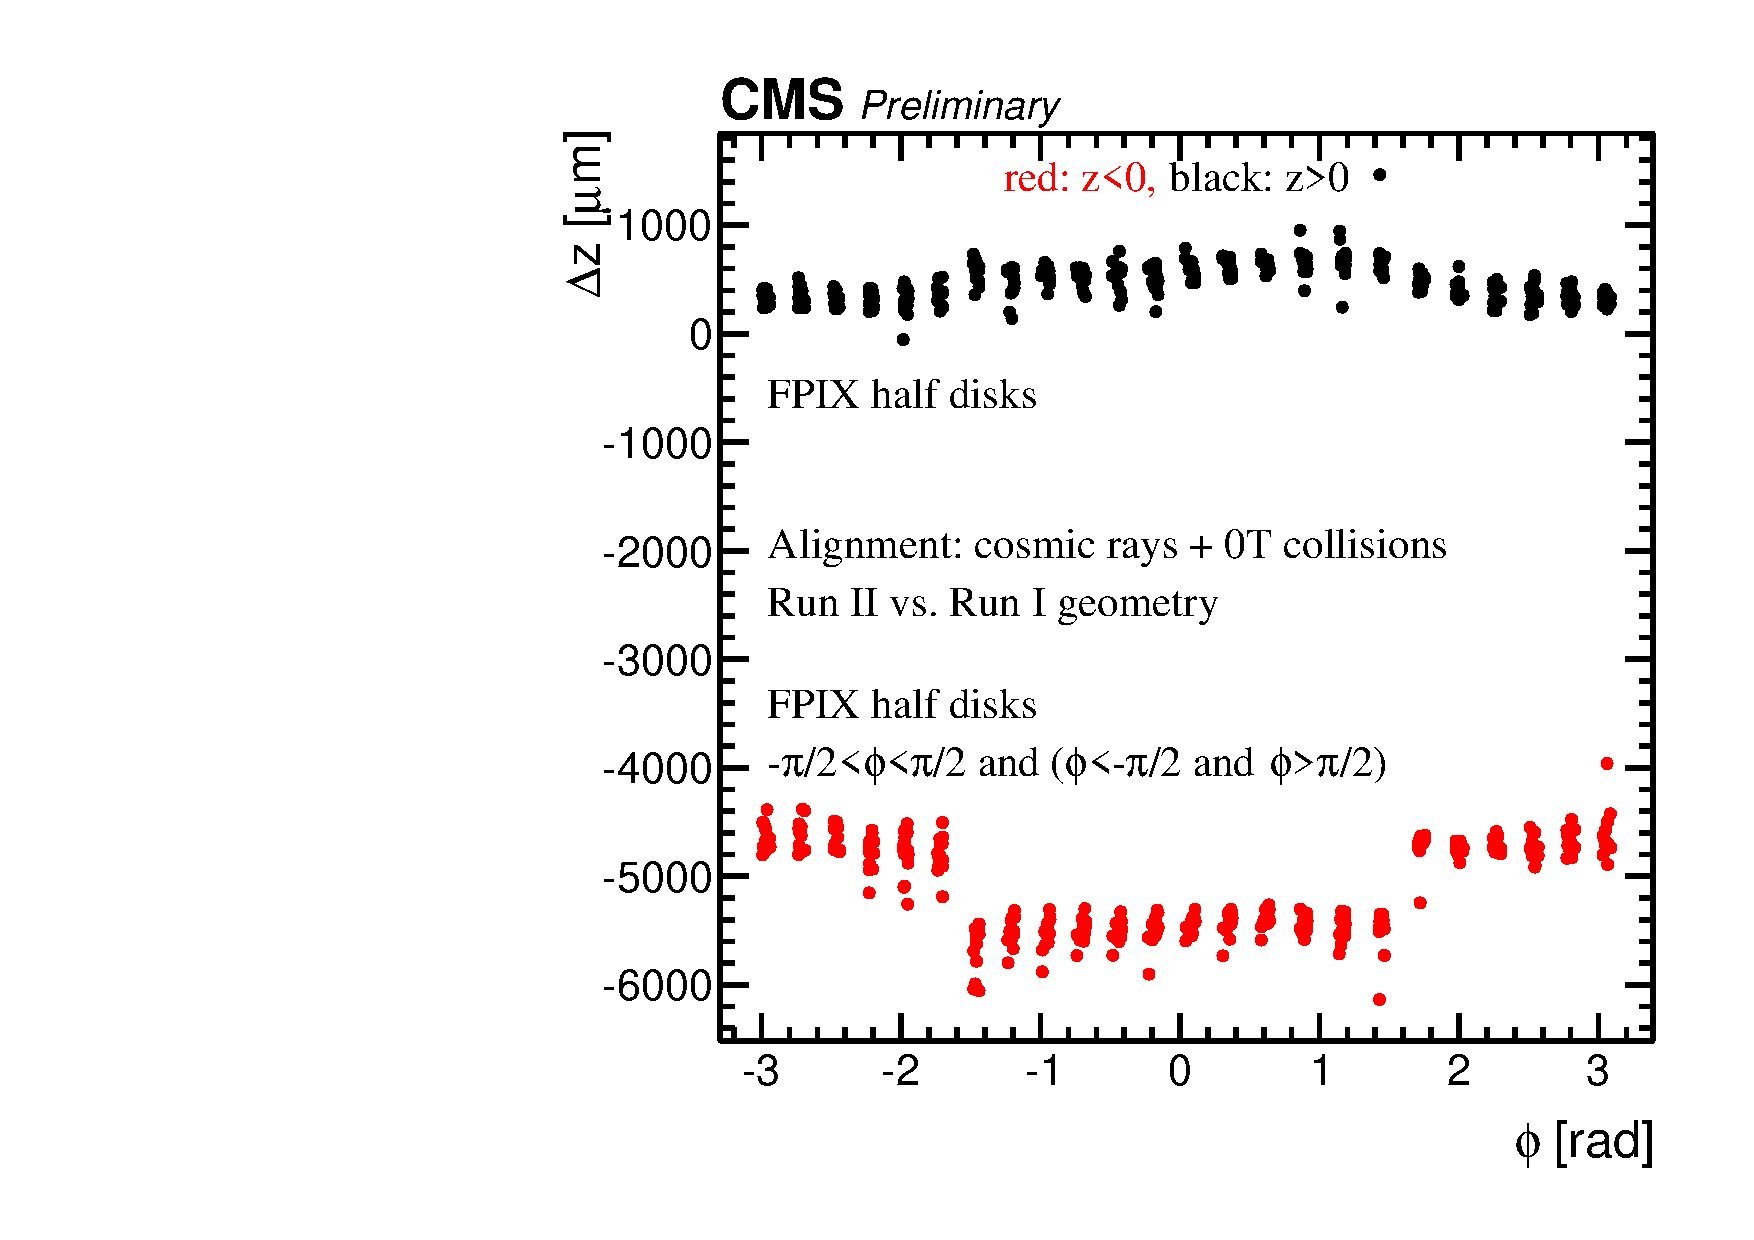
\includegraphics[width=0.45\textwidth]{../figs/Alignment/AlRes_phi_vs_dz_PXF_1.pdf}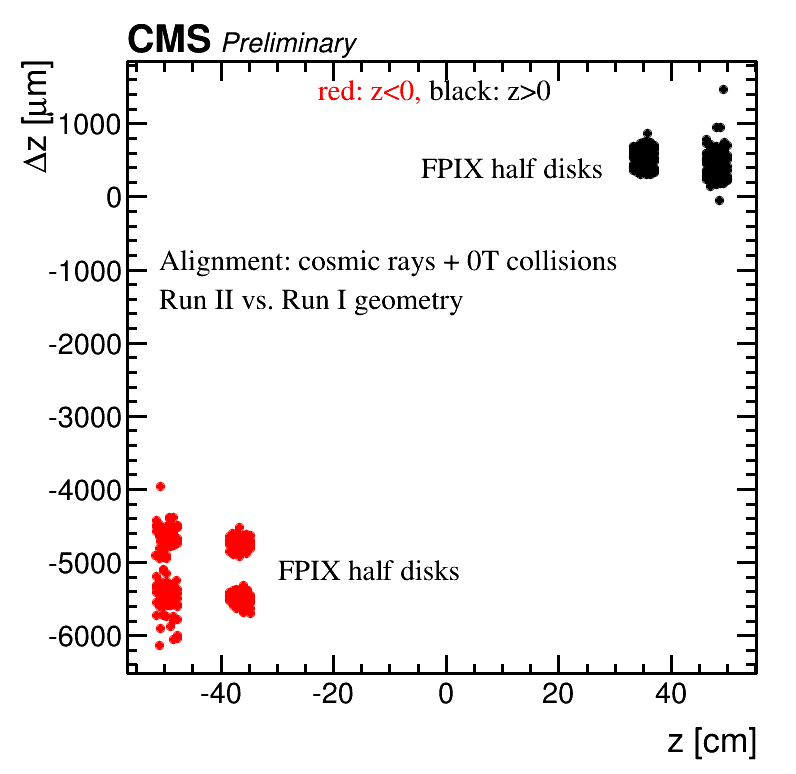
\includegraphics[width=0.45\textwidth]{../figs/Alignment/AlRes_z_vs_dz_PXF_1.png}
    \end{center}
    \caption{Comparison of Run II and Run I positions of the modules in the forward-pixel (FPIX) detector of the tracker, determined with the Millepede-II and HIP algorithms using cosmic ray data collected with 0T and 3.8T magnetic field in the solenoid. The difference $\Delta z$(Run~II~-~Run~I) as a functions of $z$ (left) and $\phi$ (right) in global coordinates. Modules in the endcap half-disks at the $-z$ side are shown in red, modules in the half-disks at the $+z$ side are shown in black.}
    \label{fig:GCP_FPIX}
\end{figure}

\begin{figure}[htb] 
    \begin{center}
        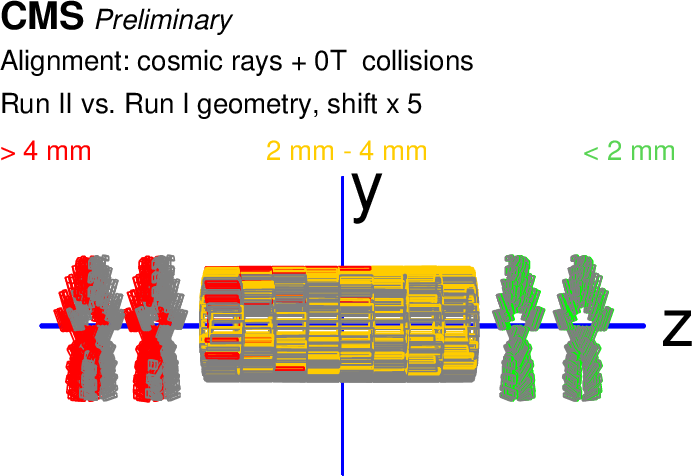
\includegraphics[width=0.95\textwidth]{../figs/Alignment/AlRes_RunIIvsRunI.png}
    \end{center}
    \caption{Geometry comparison, 3D plot of Pixel Barrel and Pixel Forward. Comparison of Run II and Run I positions of the pixel modules of the tracker, determined with the Millepede-II and HIP algorithms using cosmic ray data collected with 0T and 3.8T magnetic field in the solenoid and 0T collision data at 13 CMS.TeV. The positions at the end of Run I are shown in gray. The module shifts between Run I and Run II are magnified by a factor of 5 for visualization, and the resulting positions are shown in red, yellow, or green, depending on the magnitude of the shift. The red is mostly concentrated in the -z endcap, which moved by about 6 mm away from the barrel. The barrel is mostly yellow, as it was moved up by (-1.3,-3.38) mm in (x,y) in the re-centering procedure around the beampipe during the installation phase prior to Run II. Because of additional movements of the two half-barrels, a few modules are red. The half barrel on the +x side (direction inwards into the picture) was in addition subject of extensive repair and replacement work. }
    \label{fig:GCP_3D}
\end{figure}

\begin{figure}[htb] 
    \begin{center}
        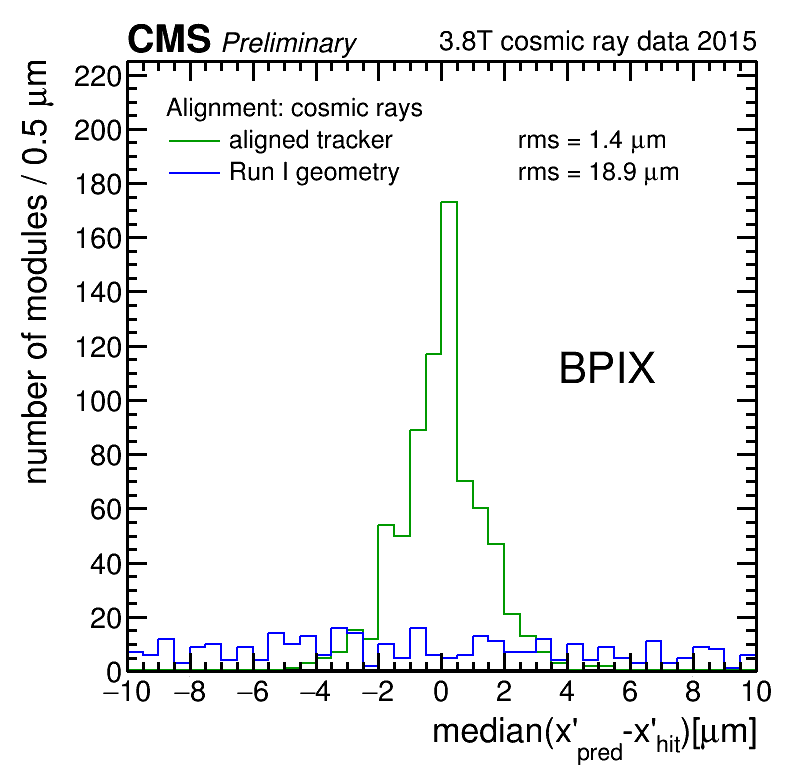
\includegraphics[width=0.45\textwidth]{../figs/Alignment/AlRes_CRAFT_DmedianR_BPIX_plain.png}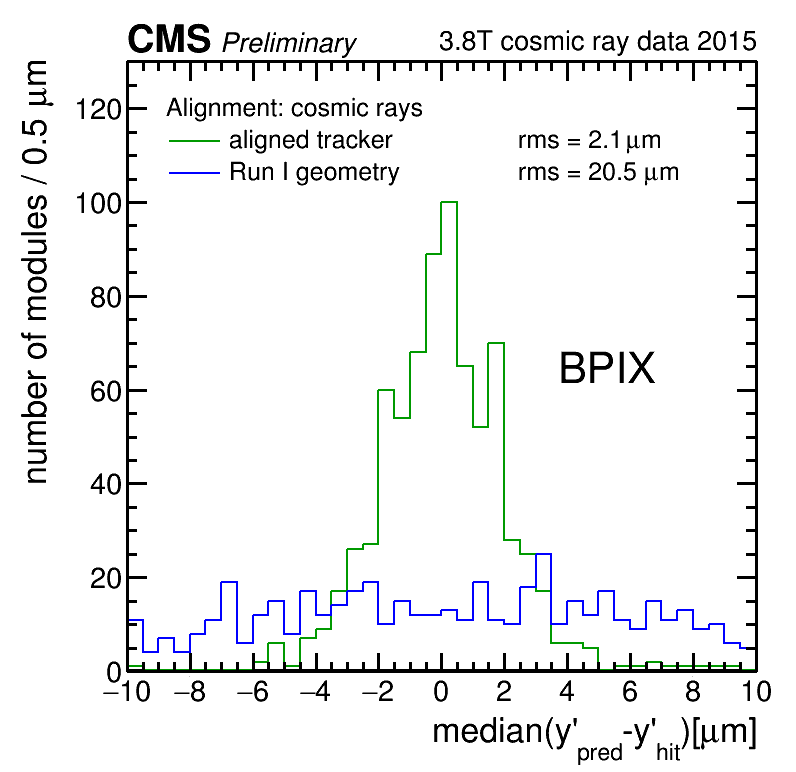
\includegraphics[width=0.45\textwidth]{../figs/Alignment/AlRes_CRAFT_DmedianYR_BPIX_plain.png}
    \end{center}
    \caption {Distributions of Median Residuals. The distribution of median residuals is plotted for the local x-direction in the barrel pixel detector, using 2 million cosmic ray tracks collected with the magnetic field at 3.8T. The blue line shows the Run I geometry, which is no longer valid for Run II data, primarily because of temperature changes and pixel re-centering and repair. The alignment shown in green was produced with the Millepede-II and HIP algorithms using 0T and 3.8T cosmic ray data. The rms values, calculated using modules both inside and outside the plot range, show improvement over the Run I geometry by a factor of 10. Right: The distribution of median residuals is plotted for the local y-direction in the barrel pixel detector, using 2 million cosmic ray tracks collected with the magnetic field at 3.8T. The blue line shows the Run I geometry, which is no longer valid for Run II data, primarily because of temperature changes and pixel re-centering and repair. The alignment shown in green was produced with the Millepede-II and HIP algorithms using 0T and 3.8T cosmic ray data. The rms values, calculated using modules both inside and outside the plot range, show improvement over the Run I geometry by a factor of 10. }
    \label{fig:DMRs}
\end{figure}

\begin{figure}[htb]
    \begin{center}
        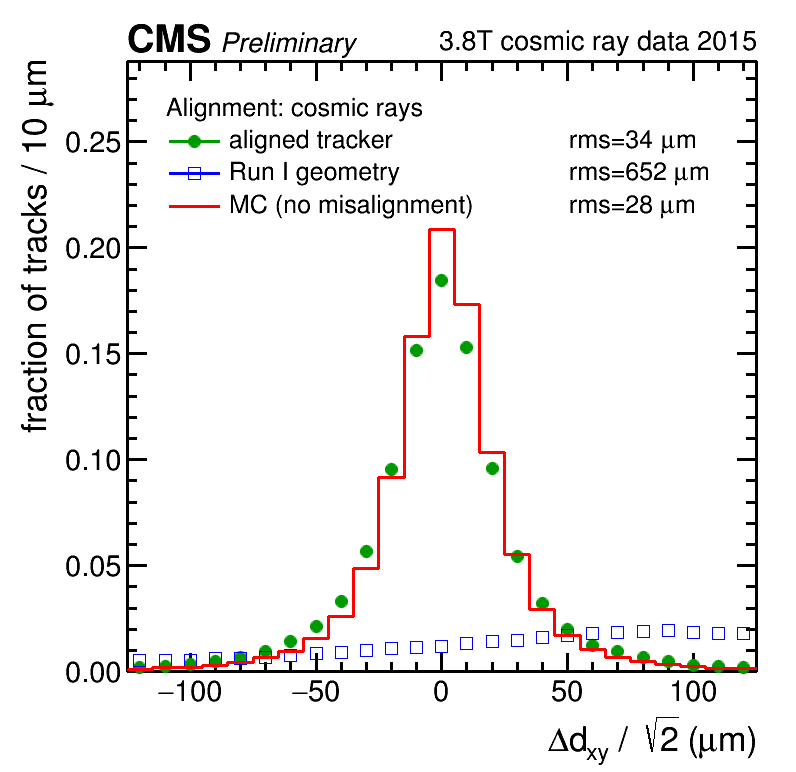
\includegraphics[width=0.45\textwidth]{../figs/Alignment/AlRes_CRAFT_hist_Delta_dxy.png}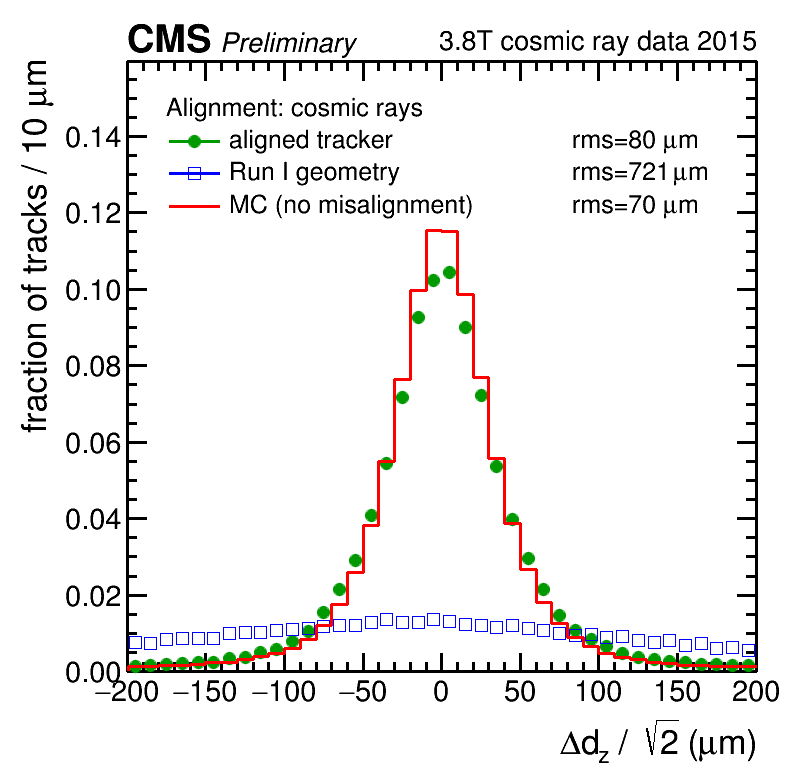
\includegraphics[width=0.45\textwidth]{../figs/Alignment/AlRes_CRAFT_hist_Delta_dz.png}
    \end{center}
    \caption{Cosmic track splitting validation. Left: The normalized differences between two halves of a cosmic track, split at the point of closest approach to the interaction region, in $d_{xy}$, the xy distance between the track and the origin. The observed precision using the aligned geometry (green circles), produced with the Millepede-II and HIP algorithms using cosmic ray data at 0 and 3.8T, is a major improvement over the Run I geometry (blue empty squares) which is no longer valid for Run II data, primarily because of temperature changes and pixel re-centering and repair. The precision comes close to that of the ideal Monte Carlo, illustrating that the tracker has almost reached its design spatial resolution. Right: The normalized differences between two halves of a cosmic track, split at the point of closest approach to the interaction region, in $d_z$, the distance in the z direction between the track and the origin. The observed precision using the aligned geometry (green circles), produced with the Millepede-II and HIP algorithms using cosmic ray data at 0 and 3.8T, is a major improvement over the Run I geometry (blue empty squares) which is no longer valid for Run II data, primarily because of temperature changes and pixel re-centering and repair. The precision comes close to that of the ideal Monte Carlo, illustrating that the tracker has almost reached its design spatial resolution. }
    \label{fig:trackSplit}
\end{figure}

\begin{figure}[htb]
    \begin{center}
        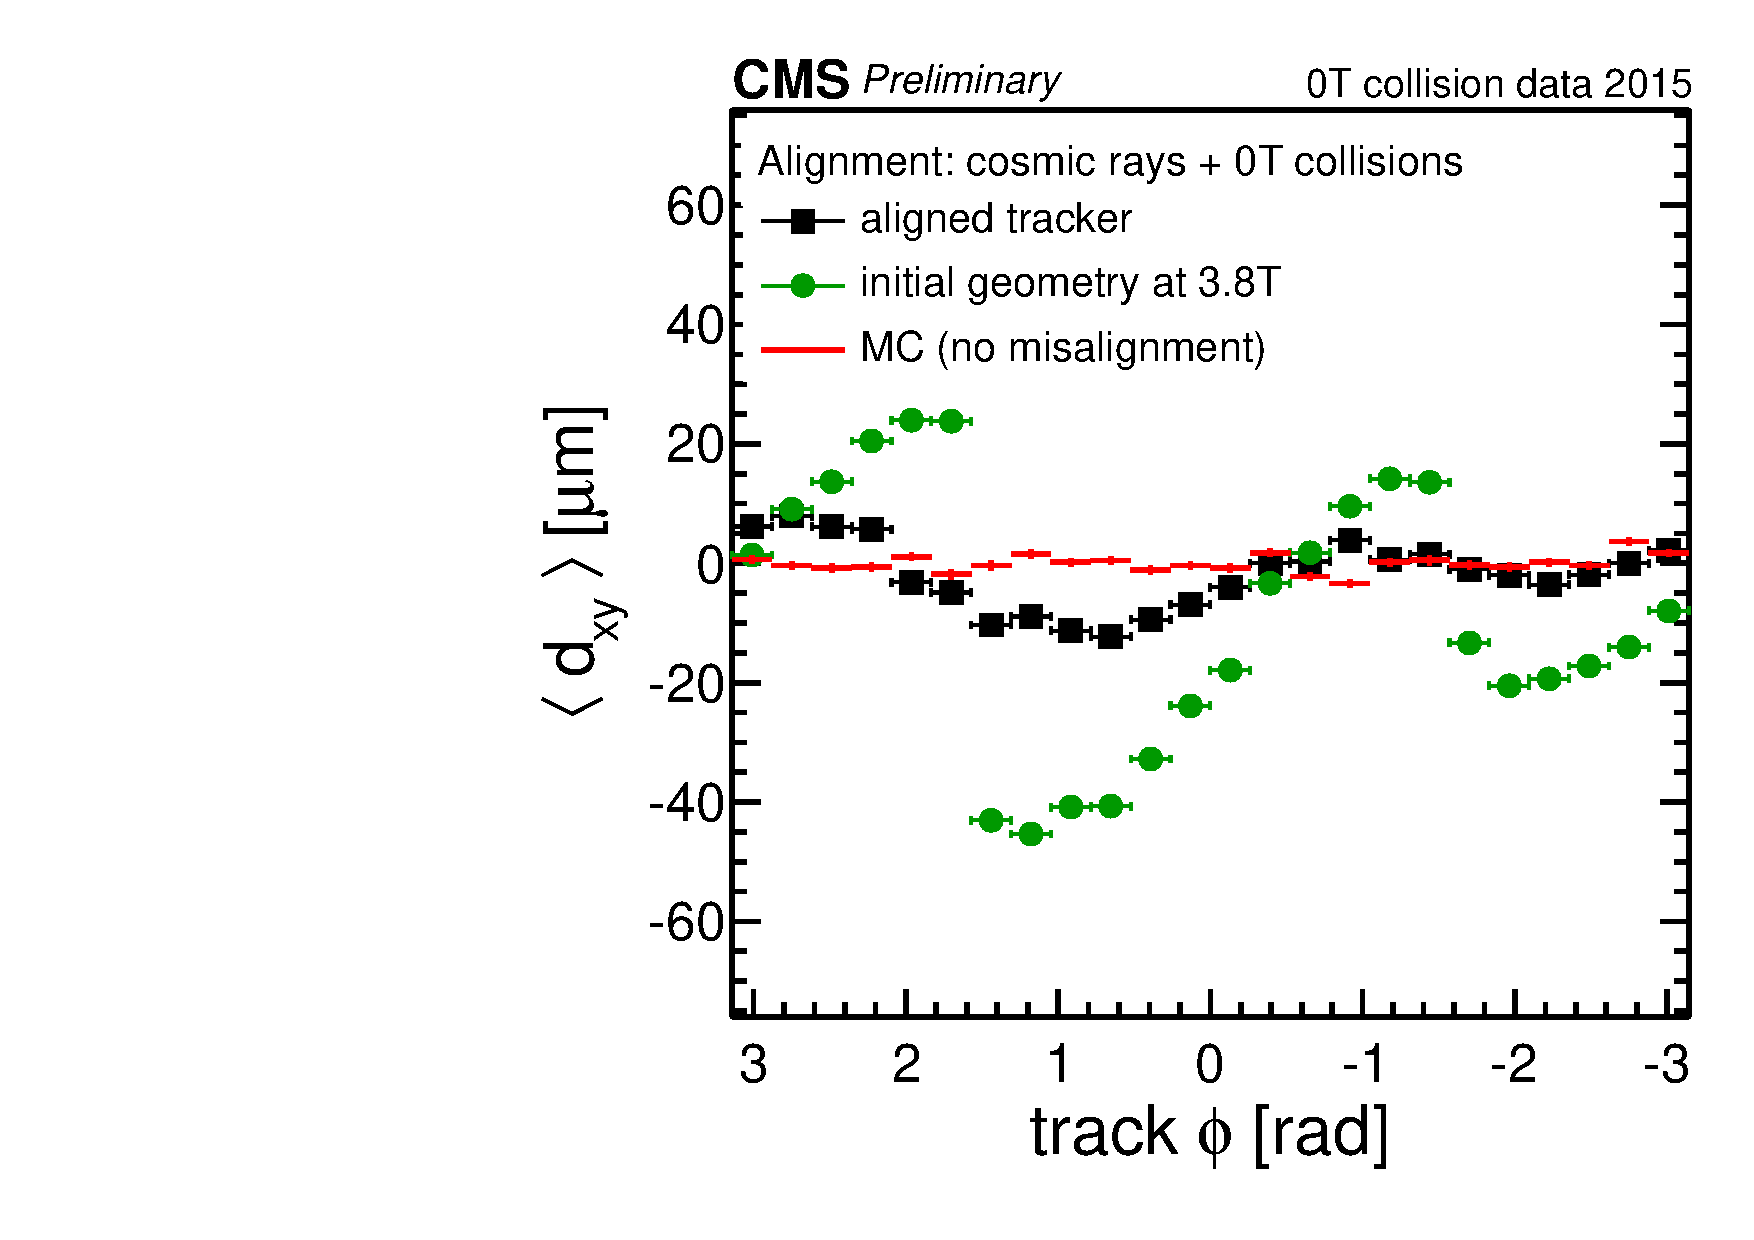
\includegraphics[width=0.45\textwidth]{../figs/Alignment/AlRes_dxyPhiBiasCanvas.pdf}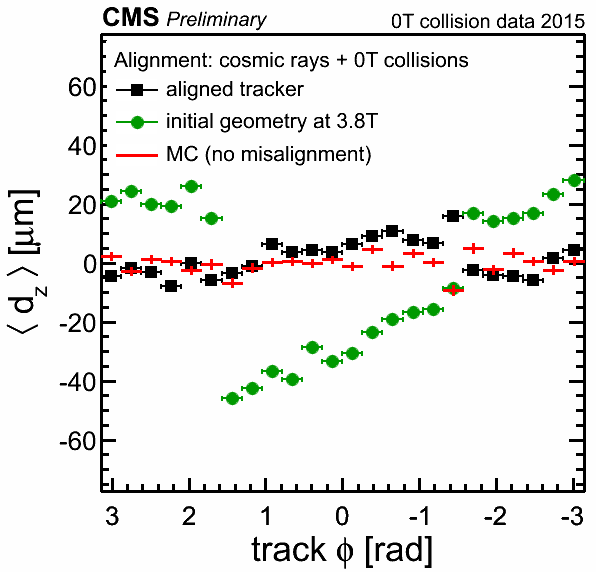
\includegraphics[width=0.45\textwidth]{../figs/Alignment/AlRes_dzPhiBiasCanvas.png}
    \end{center}
    \caption{Primary Vertex Validation. The distance in the transverse plane of the track at its closest approach to a refit unbiased primary vertex ($d_{xy}$) is studied in bins of track azimuth $\phi$ using a sample of around 5.5M events collected by the CMS detector at zero magnetic field (0T) selected online through minimum bias triggers. The performance of a dedicated alignment achieved with the Millepede-II and HIP algorithms using cosmic ray data collected with 0T and 3.8T magnetic field and 0T collision data is compared to the one of a previous alignment reached during the commissioning phase with cosmic ray tracks at full magnetic field and to a detailed detector simulation with perfect alignment and calibration. The structures of the green curve indicate relative movements of the pixel half-barrels. Right: The distance in the longitudinal plane of the track at its closest approach to a refit unbiased primary vertex ($d_{z}$) is studied in bins of track azimuth $\phi$ using a sample of around 5.5M events collected by the CMS detector at zero magnetic field (0T) selected online through minimum bias triggers. The performance of a dedicated alignment achieved with the Millepede-II and HIP algorithms using cosmic ray data collected with 0T and 3.8T magnetic field and 0T collision data is compared to the one of a previous alignment reached during the commissioning phase with cosmic ray tracks at full magnetic field and to a detailed detector simulation with perfect alignment and calibration. The structures of the green curve indicate relative movements of the pixel half-barrels. }
    \label{fig:PVvalidation}
\end{figure}

%\begin{figure}[htb]
%    \begin{center}
%        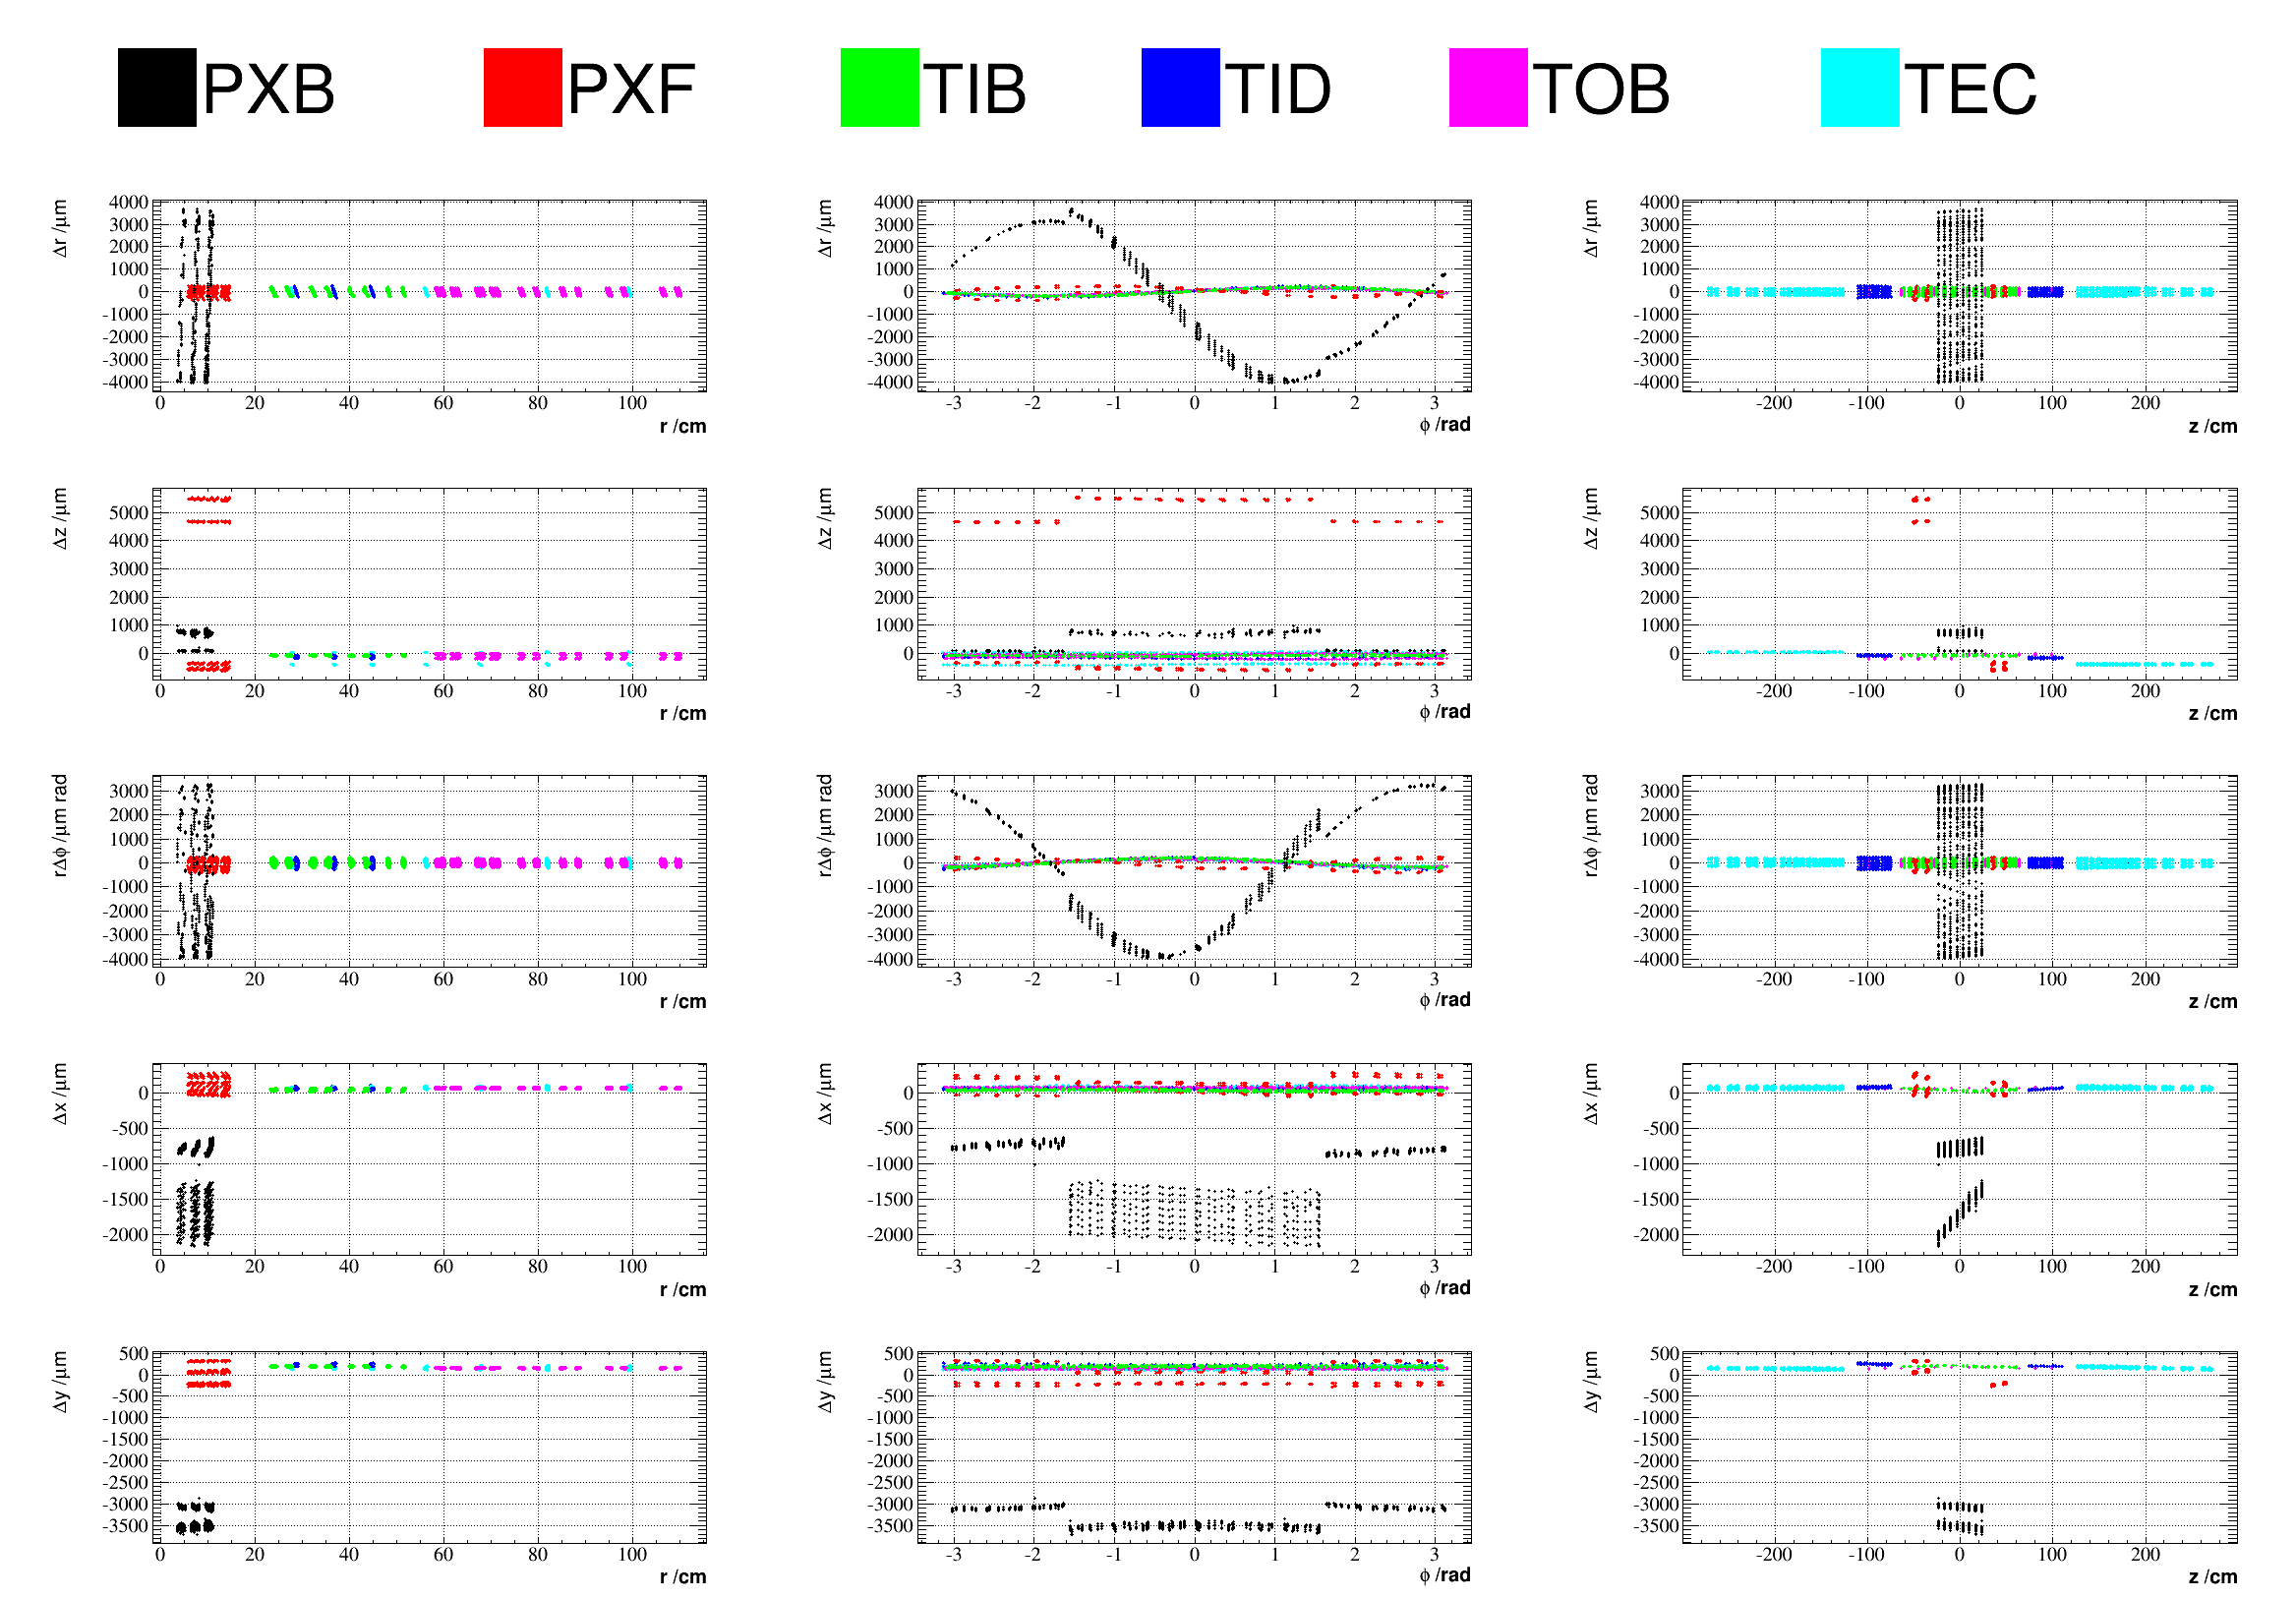
\includegraphics[width=0.98\textwidth]{../figs/Alignment/global_tracker_2_final.png}
%    \end{center}
%    \caption{Geometry comparison plot of CRUZET 2015 object vs Run I.}
%    \label{fig:trackAndResiduals}
%\end{figure}


